\section{User Interface}
This section features designs for the different areas of the system. Wireframes of each screens are provided, giving a general impression of what the screen will look like once implemented. It should be remembered, of course, that design, particularly that of a visual nature, is an iterative process, and, as such, the final product may differ, perhaps wildly, from the screens featured here.

\subsection{Colours and Typography}
As revealed through interviews conducted with staff, the school is placing a great deal of emphasis on the design of the application. As such, a unique approach to the interface will be taken, one that resonates with the new found focus on houses within the school. 

\subsubsection{Colours}
Each house has their own colour, and this colour will be used to theme all elements of the interface, depending on the house that a student is logged in as. The colour mappings are as follows:

\begin{itemize}
  \item Acton - Blue
  \item Baxter - Orange
  \item Clive - Green
  \item Darwin - Purple
  \itemm Houseman - Red
  \item Webb - Yellow
\end{itemize}

In order to ensure that each user sees a subtedly different design, even if they are in the saem house, the colours will be randomised. For example, a user in Acton might see buttons in a light blue and drop down boxes in a dark blue, whilst another user in Acton would see slightly darker or lighter shades. In order to make the system more appealing to use, the luminosity of each colour will be locked to a certain brightness.

\subsubsection{Typography}
In order to make the system yet more appealing and approachable, the font ``Dosis'' will be used throughout. As show by the example below, Dosis is a friendly font, one that invites the user to perform actions. This is in line with the objectives for the system, and will make the system suitable for all ages in the school.

\subsection{Login Screen}
\begin{figure}[h!]
  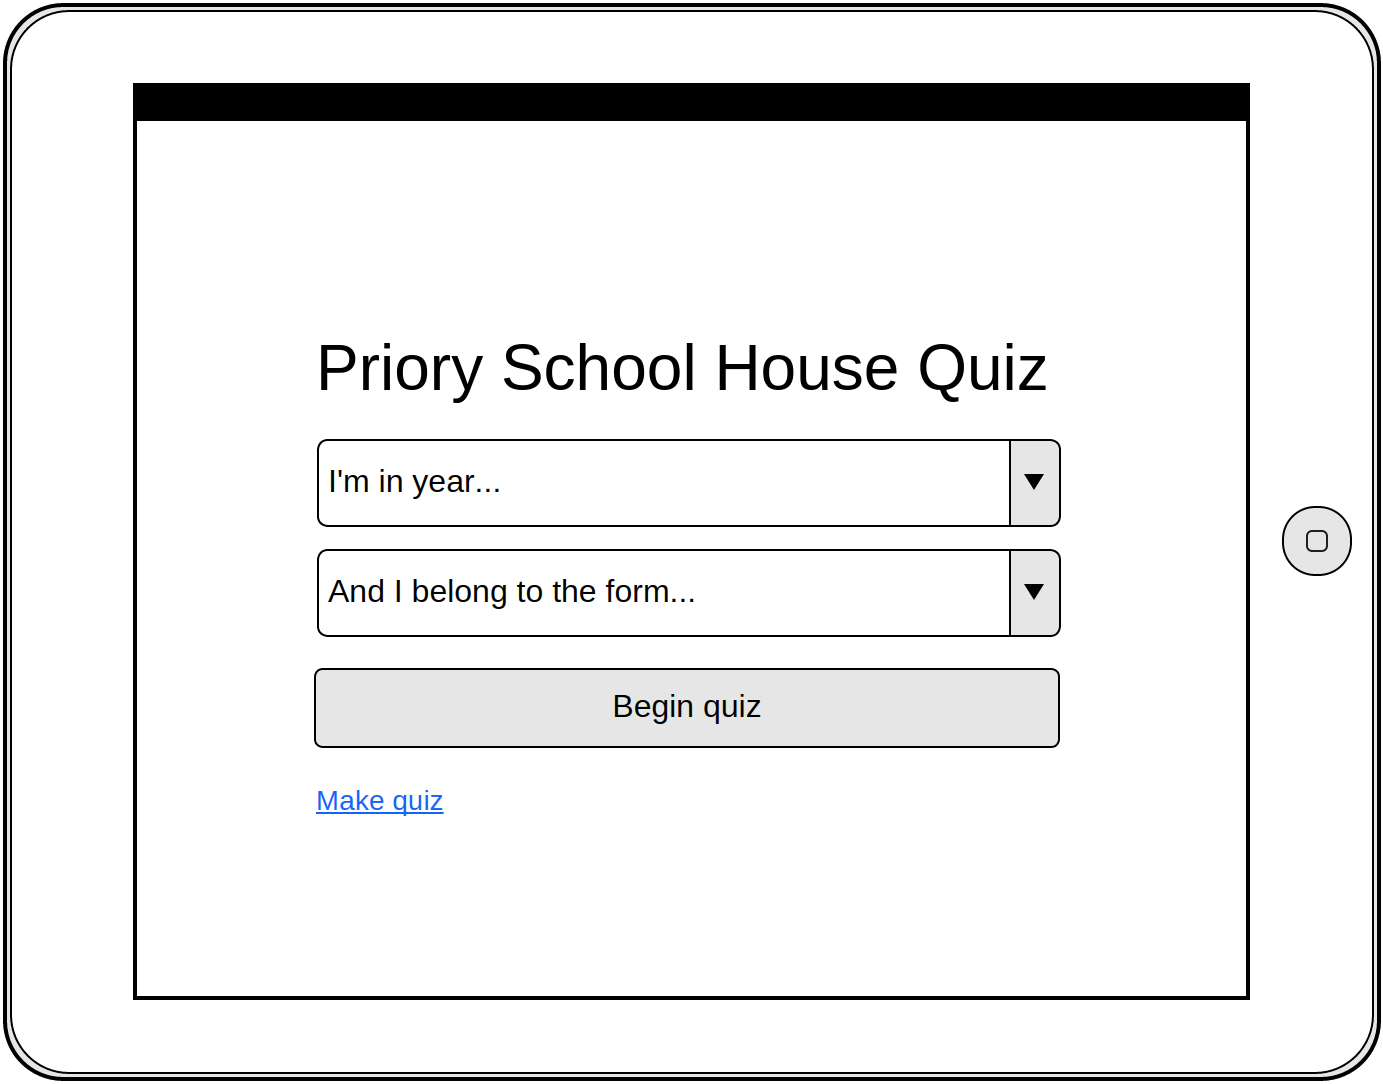
\includegraphics[scale=0.24]{design/login}
\end{figure}

Due to the way the school names individual form groups, a simplified approach to the login form can be used. Two drop down boxes will be used, one for the year - containing the items 7, 8, 9, 10 and 11 - and one for the house - Acton, Baxter, Clive, Darwin, Houseman, Webb. By doing this, any combination of form group can be computed. Interviews with students revealed that they would not be likely to pose as a member of another form group, so no authentication is needed - students need simply enter their year group and house, and then press the ``Begin quiz'' button. If a senior member of staff needs to create a quiz, clicking the link will bring them to a password prompt, in order to prevent errant students making a quiz themselves. Because the user will not have chosen their house, house colours will not be available. Instead, the colours of all the houses will feature, with the interface elements changing every few seconds to the next house.

\clearpage

\subsection{Countdown Screen}
\begin{figure}[h!]
  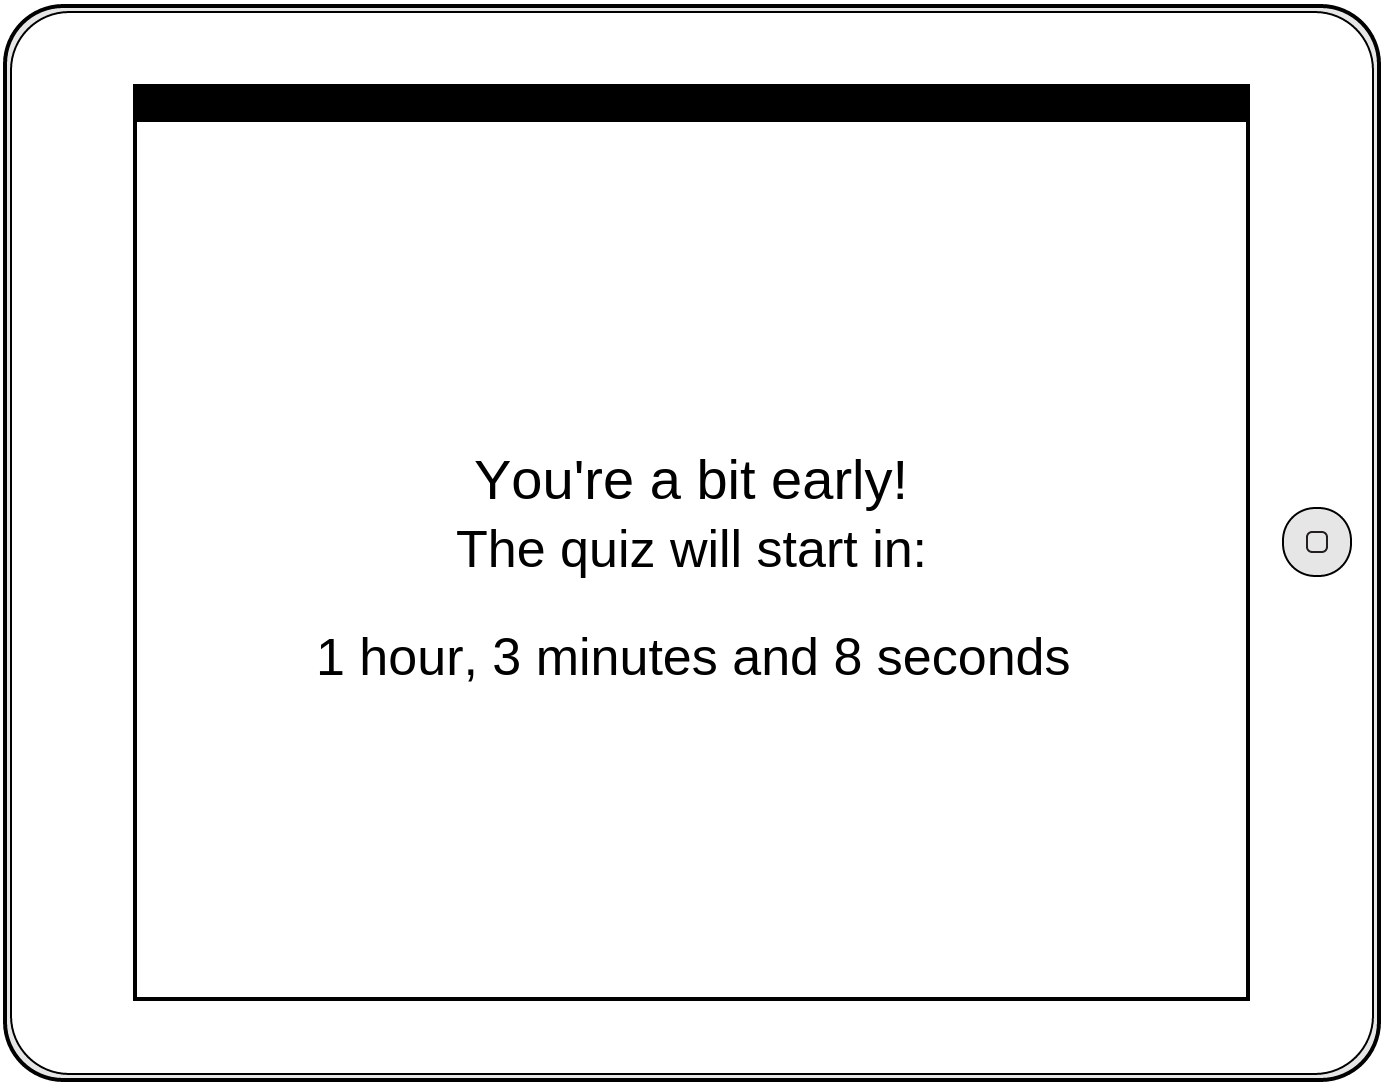
\includegraphics[scale=0.24]{design/countdown}
\end{figure}

In the event that a student logs onto the system and a quiz is yet to start, this screen will be displayed, informing them how long they have to wait. The countdown timer will display the time till the next scheduled quiz in hours, minutes and seconds, and will update accordingly.

\clearpage

\subsection{Quiz Creation Screen}
\begin{figure}[h!]
  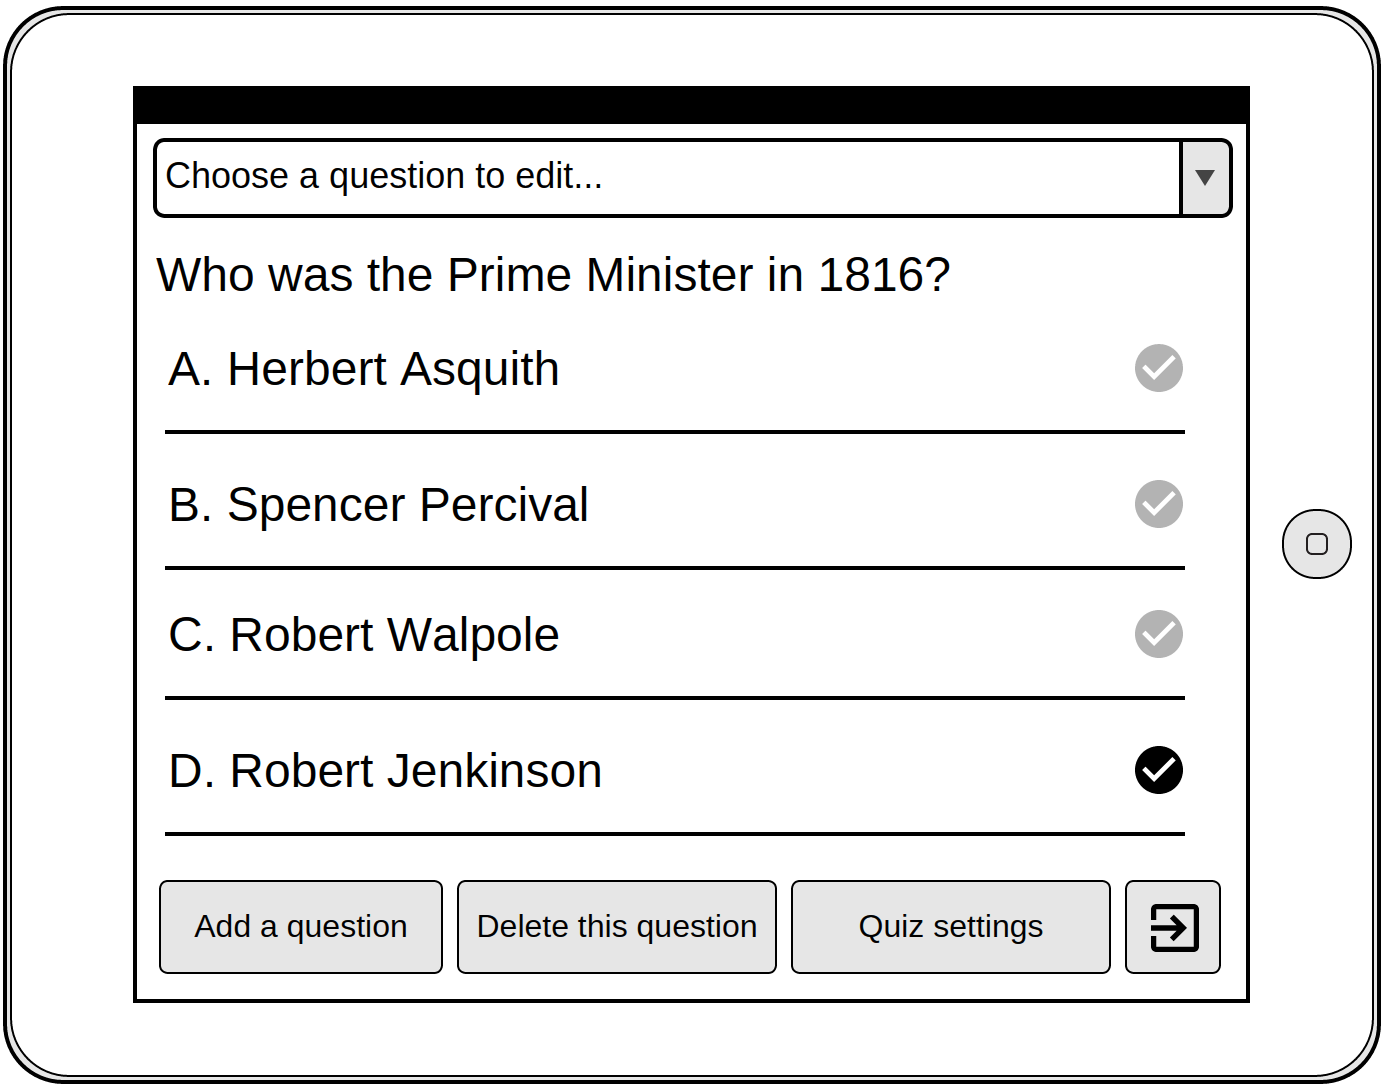
\includegraphics[scale=0.24]{design/quiz_maker}
\end{figure}

\clearpage

\subsection{Play Quiz Screen}
\begin{figure}[h!]
  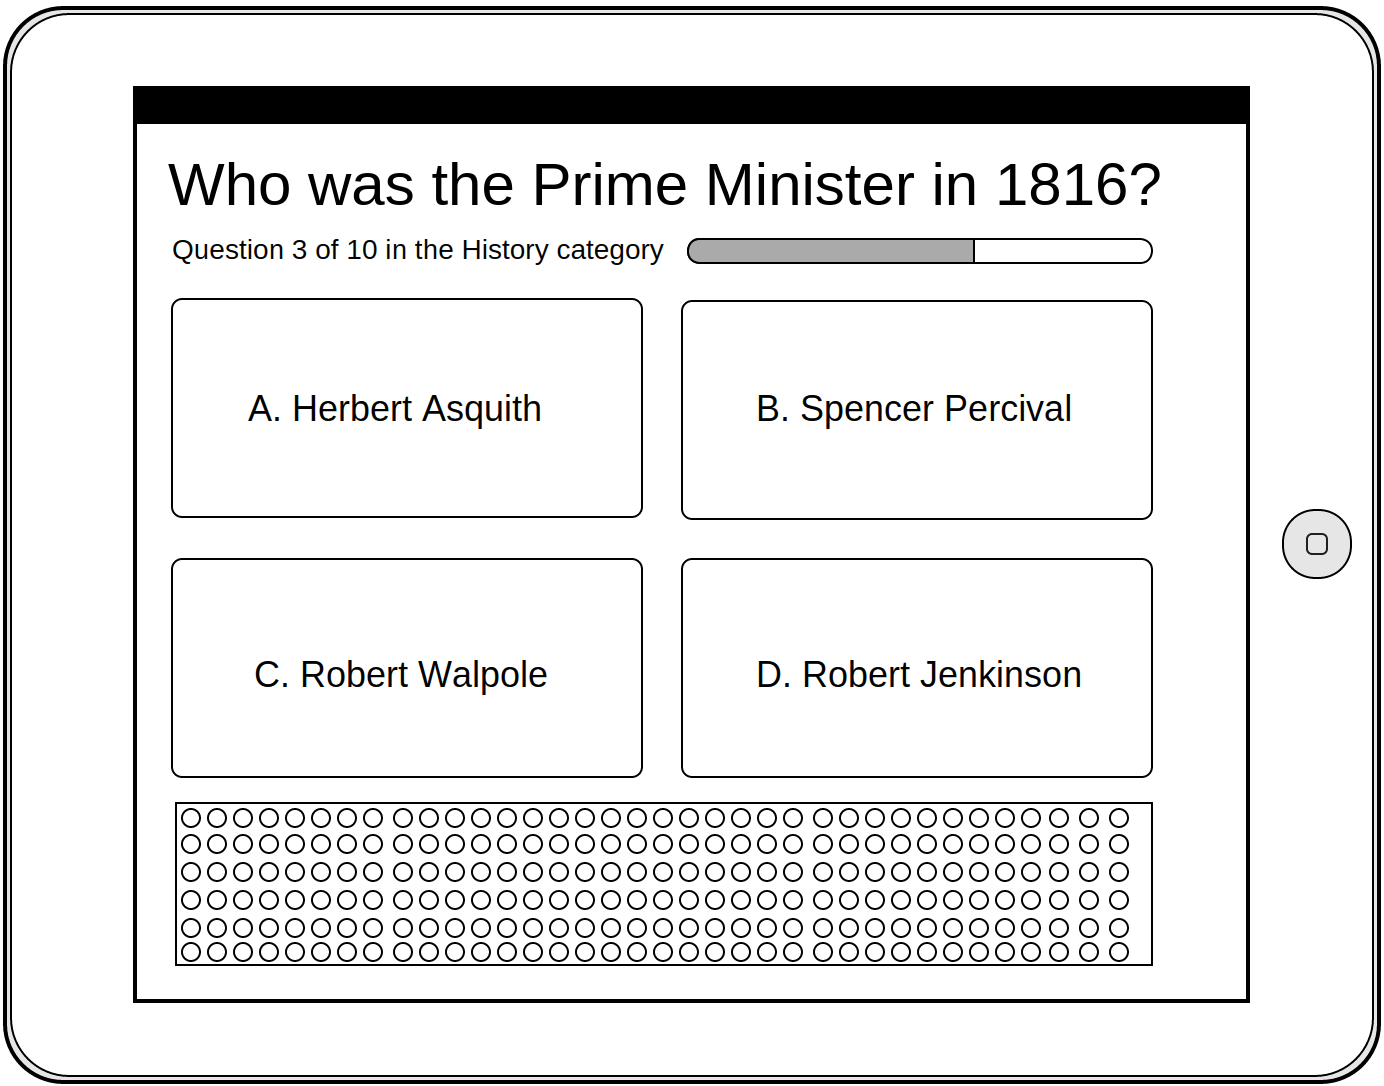
\includegraphics[scale=0.24]{design/quiz_play}
\end{figure}
